\documentclass[12pt]{article}
\usepackage{amsmath}
\usepackage{amssymb}
\usepackage{cancel}
\usepackage{graphicx}
% \usepackage{physics}
\usepackage{siunitx}
\usepackage{wrapfig}

% \AtBeginDocument{\RenewCommandCopy\qty\SI}

\newcommand{\E}[1]{\times 10^{#1}}

\title{
    Chapter 33 End-of-Chapter Problems
    \\ \small
    Halliday \& Resnick, 10th Edition
}

\author{Donald Aingworth IV}

\date{\small Hit me where it Matters}

\begin{document}
    \DeclareSIUnit{\atm}{atm}
    \DeclareSIUnit{\cal}{\ cal}
    \DeclareSIUnit{\Cal}{\ Cal}
    \DeclareSIUnit{\calorie}{\ cal}
    \DeclareSIUnit{\Calorie}{\ Cal}
    \DeclareSIUnit{\celsiusdegree}{C^\circ}
    \DeclareSIUnit{\fahrenheit}{^\circ F}
    \DeclareSIUnit{\fahrenheitdegree}{F^\circ}
    \DeclareSIUnit{\torr}{\ torr}

    \maketitle

    \pagebreak
    \section{Problem 1}
        A certain helium-neon laser emits red light in a narrow band of wavelengths centered at 632.8 nm and with a “wavelength width” (such as on the scale of Fig. 33-1) of 0.0100 nm. 
        What is the corresponding “frequency width” for the emission?

        \subsection{Solution}
            Use the traditional formula for the wavelength.
            Here, the speed of the wave is the speed of light.
            We can treat this like an error and raw value issue.
            \begin{gather}
                v   =   \lambda f   \to
                f   =   \frac{c}{\lambda}\\
                \frac{\delta f}{f} = \frac{\delta \lambda}{\lambda}\\
                \begin{align}
                    \delta f    &=  f * \frac{\delta \lambda}{\lambda}
                        =   c * \frac{\delta \lambda}{\lambda^2}\\
                        &=  2.998\E{8}\,\unit{\meter/\second} * \frac{0.0100\,\unit{\nano\meter}}{(632.8\,\unit{\nano\meter})^2}\\
                        &=  \boxed{7.49\,\unit{\giga\hertz}}
                \end{align}
            \end{gather}

    \pagebreak
    \section{Problem 5}
        What inductance must be connected to a 17 pF capacitor in an oscillator capable of generating 550 nm (i.e., visible) electromagnetic waves? 
        Comment on your answer.

        \subsection{Solution}
            For an $LC$ circuit, the angular frequency is $\frac{1}{\sqrt{LC}}$.
            \begin{equation}
                \omega  =   \frac{1}{\sqrt{LC}}
            \end{equation}

            The linear frequency is calculatable from this.
            \begin{equation}
                f   =   \frac{\omega}{2\pi}
                    =   \frac{1}{2\pi\sqrt{LC}}
            \end{equation}

            This can be relatable to the wave speed (the speed of light in the case of an EM wave).
            \begin{gather}
                v   =   \lambda f\\
                c   =   \lambda f
                    =   \frac{\lambda}{2\pi\sqrt{LC}}
            \end{gather}

            Ths can be solved for the inductance ($L$) and found a solution for.
            \begin{gather}
                c   =   \frac{\lambda}{2\pi\sqrt{L}\,\sqrt{C}}\\
                \sqrt{L}    =   \frac{\lambda}{2\pi c\sqrt{C}}\\
                \begin{align}
                    L   &=  \frac{\lambda^2}{(2\pi)^2 c^2 C}\\
                        &=  \frac{(550\,\unit{\nano\meter})^2}{4\pi^2 (2.998\E{8}\,\unit{\meter/\second})^2 * 17\,\unit{\pico\farad}}\\
                        &=  \boxed{5.015\E{-21}\,\unit{\henry}}
                \end{align}
            \end{gather}

    \pagebreak
    \section{Problem 7}
        What is the intensity of a traveling plane electromagnetic wave if $B_m$ is $1.0\E{-4}\,\unit{\tesla}$?

        \subsection{Solution}
            Start by calculating the electric wave magnitude.
            \begin{gather}
                c   =   \frac{E_m}{B_m}\\
                E_m =   c\,B_m
                    =   2.998\E{8}\,\unit{\meter/\second} * 1.0\E{-4}\,\unit{\tesla}
                    =   2.998\E{4}\,\unit{\newton/\coulomb}
            \end{gather}

            The intensity can be calculated from this.
            Bear in mind that $E_{\rm rms} = \frac{E_m}{\sqrt{2}}$.
            \begin{align}
                I   &=  \frac{1}{c \mu_0} E_{\rm rms}^2
                    =   \frac{E_m^2}{2c \mu_0}
                    =   \frac{c B_m^2}{2\mu_0}\\
                    &=  \frac{2.998\E{8}\,\unit{\meter/\second} * 10^{-8}\,\unit{\tesla^2}}{2*1.257\E{-6}\,\unit{\henry/\meter}}\\
                    &=  \boxed{1.193\E{6}\,\unit{\watt/\meter}}
            \end{align}

    % \pagebreak
    \section{Problem 9}
        Some neodymium-glass lasers can provide $100\,\unit{\tera\watt}$ of power in 1.0 ns pulses at a wavelength of 0.26 \unit{\micro\meter}. 
        How much energy is contained in a single pulse?

        \subsection{Solution}
            Multiply the power of the laser by the frequency of the pulses to get the energy of a single pulse.
            \begin{equation}
                E   =   P * f
                    =   100\E{12}\,\unit{\watt} * 1.0\E{-9}\,\unit{\second}
                    =   \boxed{100\,\unit{\kilo\joule}}
            \end{equation}

    \pagebreak
    \section{Problem 11}
        A plane electromagnetic wave traveling in the positive direction of an x axis in vacuum has components $E_x = E_y = 0$ and $E_z$ has the below value. 
        \begin{equation}
            E_z = (2.0\,\unit{\volt/\meter})\cos\left[ (\pi \E{15}\,\unit{\second^{-1}})(t - x/c) \right] 
        \end{equation}
        (a) What is the amplitude of the magnetic field component? 
        (b) Parallel to which axis does the magnetic field oscillate? 
        (c) When the electric field component is in the positive direction of the z axis at a certain point P, what is the direction of the magnetic field component there?

        \subsection{Solution (a)}
            The amplitude would be proportional to the electric field component and the speed of light.
            \begin{equation}
                B_m =   \frac{E_m}{c}
                    =   \frac{2.0\,\unit{\volt/\meter}}{2.998\E{8}\,\unit{\meter/\second}}
                    =   \boxed{6.67\E{-9}\,\unit{\tesla}}
            \end{equation}

        \subsection{Solution (b)}
            It would also depend on the $x$-value so it would not be parallel to the $x$ axis.
            It can't be parallel to the $z$ axis because the electric field already is.
            The only axis left is the \boxed{y} axis.

        \subsection{Solution (c)}
            The the magnetic wave along its axis is negatively proportional to the magnitude of the electric wave on its axis.
            As such, if the electric wave is in the positive direction of the $z$ axis, then the magnetic wave will be in the \boxed{\text{negative $y$-direction}}.

    \pagebreak
    \section{Problem 13}
        Sunlight just outside Earth's atmosphere has an intensity of 1.40 \unit{\kilo\watt/\meter^2}. 
        Calculate (a) $E_m$ and (b) $B_m$ for sunlight there, assuming it to be a plane wave.

        \subsection{Solution (a)}
            The magnitude of the electric field is calculatable from the intensity.
            Start with the RMS electric field and the intensity.
            \begin{equation}
                I = \frac{1}{c \mu_0} E_{rms}^2
            \end{equation}

            The relationship with the magnitude of the electric field and the RMS electric field ($E_{rms}^2 = \frac{E_m^2}{2}$) can be applied here.
            \begin{equation}
                I = \frac{E_m^2}{2c\mu_0}
            \end{equation}

            This can be solved for $E_m$ to find its value.
            \begin{align}
                E_m &=  \sqrt{2Ic\mu_0}\\
                    &=  \sqrt{2 * 1.40\E{3}\,\unit{\watt/\meter^2} * 2.998\E{8}\,\unit{\meter/\second} * 1.257\E{-6}\,\unit{\henry/\meter}}\\
                    &=  \sqrt{1.055\E{6}\,\unit{\newton^2/\coulomb^2}}
                    =   \boxed{1027\,\unit{\newton/\coulomb}}
            \end{align}

        \subsection{Solution (b)}
            Use the fraction for electromagnetic waves related to the speed of light.
            \begin{equation}
                c   =   \frac{E_m}{B_m}
            \end{equation}

            Solve for and find the magnitude of the magnetic wave.
            \begin{align}
                B_m &=  \frac{E_m}{c}
                    =   \frac{1027\,\unit{\newton/\coulomb}}{2.998\E{8}\,\unit{\meter/\second}}\\
                    &=  \boxed{3.426\E{-6}\,\unit{\tesla}}
            \end{align}

    \pagebreak
    \section{Problem 19}
        High-power lasers are used to compress a plasma (a gas of charged particles) by radiation pressure. 
        A laser generating radiation pulses with peak power $1.5\E{3}$ MW is focused onto 1.0 \unit{\milli\meter^2} of high-electron-density plasma. 
        Find the pressure exerted on the plasma if the plasma reflects all the light beams directly back along their paths.

        \subsection{Solution}
            The power would be equivalent to the intensity multiplied by the area impacted.
            \begin{equation}
                P = IA \leftrightarrow I = \frac{P}{A}
            \end{equation}

            This in turn can be used in the equation for pressure (and force) from radiation.
            Bear in mind that since the plasma reflects all light rays, we would use the corresponding equation.
            \begin{align}
                p_r &=  \frac{2I}{c}
                    =   \frac{2P}{cA}
                    =   \frac{2 * 1.5\E{9}\,\unit{\watt}}{(2.998\E{8}\,\unit{\meter/\second})(1.0\E{-6}\,\unit{\meter^2})}\\
                    &=  \boxed{1.0\E{7}\,\unit{\pascal}}
            \end{align}

    \pagebreak
    \section{Problem 21}
        What is the radiation pressure 1.5 m away from a 500 W lightbulb? 
        Assume that the surface on which the pressure is exerted faces the bulb and is perfectly absorbing and that the bulb radiates uniformly in all directions.

        \subsection{Solution}
            Radiation pressure is equal to the intensity divided by the speed of light.
            \begin{equation}
                p_r = \frac{I}{c}
            \end{equation}

            The intensity is equal to the power divided by the area affected.
            \begin{equation}
                I = \frac{P}{A} = \frac{P}{4\pi r^2}
            \end{equation}

            This can be applied to find the radiation pressure.
            \begin{align}
                p_r &=  \frac{I}{c}
                    =   \frac{\frac{P}{4\pi r^2}}{c}
                    =   \frac{P}{4\pi r^2 c}\\
                    &=  \frac{500\,\unit{\watt}}{4\pi * (1.5\,\unit{\meter})^2 * 2.998\E{8}\,\unit{\meter/\second}}\\
                    &=  \boxed{5.899\E{-8}\,\unit{\pascal}}
            \end{align}

    \pagebreak
    \section{Problem 29}
        A small spaceship with a mass of only $1.5\E{3}$ kg (including an astronaut) is drifting in outer space with negligible gravitational forces acting on it. 
        If the astronaut turns on a 10 kW laser beam, what speed will the ship attain in 1.0 day because of the momentum carried away by the beam?

        \subsection{Solution}
            To begin, there are 86400 seconds in a day.
            Multiply this by the 10 kW, we wind up with $8.64\E{8}\,\unit{\joule}$ lost or gained from the laser in one day.
            Divide this energy by the speed of light to get the momentum added, which we then divide by the mass to get the speed increase.
            \begin{align}
                \Delta p    &=  \frac{\Delta U}{c}
                    =   \frac{8.64\E{8}\,\unit{\joule}}{2.998\E{8}\,\unit{\meter/\second}}
                    =   2.882\,\unit{\newton\cdot\second}\\
                \Delta v    &=  \frac{\Delta p}{m}
                    =   \boxed{0.00192\,\unit{\meter/\second}}
            \end{align}

    \pagebreak
    \section{Problem 33}
        \begin{wrapfigure}{r}{0.33\textwidth}
            \vspace{-30pt}
            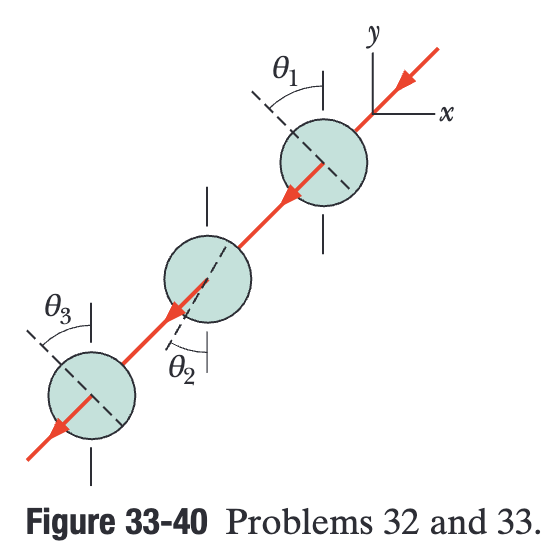
\includegraphics[width=0.33\textwidth]{33-40.png} 
            % \label{fig:wrapfig}
        \end{wrapfigure}
        In Fig. 33-40, initially unpolarized light is sent into a system of three polarizing sheets whose polarizing directions make angles of $\theta_1 = 40\unit{\degree}, \theta_2 = 20\unit{\degree}$, and $\theta_3 = 40\unit{\degree}$ with the direction of the y axis. 
        What percentage of the light's initial intensity is transmitted by the system? 
        (Hint: Be careful with the angles.)

        \subsection{Solution}
            First, it would travel through the first polarizing sheet.
            This would polarize it and cut the intensity in half.
            \begin{equation}
                I_1 = \frac{1}{2}I_0
            \end{equation}

            Next, it would travel through the second polarization disk.
            Since this makes an angle of 20\unit{\degree} with the horizontal, which itslef makes an angle of 40\unit{\degree} with the prior polarizer, 60\unit{\degree} would be our value of $\theta_2$.
            \begin{equation}
                I_2 = I_1 \cos^2(60\unit{\degree}) = \frac{1}{2}I_0 \cos^2(60\unit{\degree})
            \end{equation}

            Last, it would travel through the second polarization disk.
            Here, 60\unit{\degree} would again be our value of $\theta_2$.
            \begin{equation}
                I_3 = I_2 \cos^2(60\unit{\degree}) = \frac{1}{2}I_0 \cos^2(60\unit{\degree}) \cos^2(60\unit{\degree}) = 0.03125 I_0
            \end{equation}

            Therefore, the percentage transmitted is \boxed{3.1\%}. 
            

    \pagebreak
    \section{Problem 37}
        We want to rotate the direction of polarization of a beam of polarized light through 90\unit{\degree} by sending the beam through one or more polarizing sheets. 
        (a) What is the minimum number of sheets required? 
        (b) What is the minimum number of sheets required if the transmitted intensity is to be more than 60\% of the original intensity?

        \subsection{Solution}
            We would only need \boxed{two} sheets, one at 45\unit{\degree} and one again at 45\unit{\degree}.

        \subsection{Solution (b)}
            Assume all sheets are equally angularly spaced.
            This would mean that the angle would be, for $n$ sheets, $\frac{\pi}{2n}$.
            Furthermore, for one sheet, the intensity reduces to $\cos^2(\theta)$ the original.
            That means that for $n$ sheets, the intensity would reduce to $\cos^{2n}(\theta)$ of the original.
            Putting these together, we can solve for $n$ (or try to), setting the other side to be equal to $0.6$.
            \begin{gather}
                \cos^{2n}\left( \frac{\pi}{2n} \right) = 0.6\\
                \cos\left( \frac{\pi}{2n} \right) = 0.6^{\frac{1}{2n}}
            \end{gather}

            Let's just use guess and check.
            First $n = 2$:
            \begin{align}
                \cos^{4}\left( \frac{\pi}{4} \right) = 0.25 < 0.6
            \end{align}

            $n = 3$:
            \begin{align}
                \cos^{6}\left( \frac{\pi}{6} \right) = 0.42 < 0.6
            \end{align}

            $n = 4$:
            \begin{align}
                \cos^{8}\left( \frac{\pi}{8} \right) = 0.53 < 0.6
            \end{align}

            $n = 5$:
            \begin{align}
                \cos^{10}\left( \frac{\pi}{10} \right) = 0.605 \geq 0.6
            \end{align}

            Conclusicely, the answer is \boxed{5}. 

        \subsection{My failed attempt to solve (b) without guess and check}
            Here, we will turn this into complex form. 
            There will be an imaginary part to this.
            Since this would be the cosine of it, we could use the pythagorean theorem by assuming a 3-4-5 triangle and finding the other edge will have an edge length of $0.8$.
            \begin{gather}
                e^{\frac{i\pi}{2n}} = 0.6^{\frac{1}{2n}} + i 0.8^{\frac{1}{2n}}
            \end{gather}

            Convert the right side to complex form.
            \begin{equation}
                e^{\frac{i\pi}{2n}} = e^{i \frac{\arctan(4/3)}{2n}}
            \end{equation}

            Take the naural log of everything, then divide everything by $i$. 
            \begin{equation}
                \frac{\pi}{2n} = \frac{\arctan(4/3)}{2n}
            \end{equation}

    \pagebreak
    \section{Problem 41}
        A beam of polarized light is sent into a system of two polarizing sheets. 
        Relative to the polarization direction of that incident light, the polarizing directions of the sheets are at angles $\theta$ for the first sheet and 90\unit{\degree} for the second sheet. 
        If 0.10 of the incident intensity is transmitted by the two sheets, what is $\theta$?

        \subsection{Solution}
            This requires an equation to take in both polarizations.
            \begin{equation}
                I = I_0 \cos^2 (\theta) \cos^2 \left( \frac{\pi}{2} - \theta \right)
            \end{equation}

            We can use the trig identity of $\cos\left( \frac{\pi}{2} - \theta \right) = \sin(\theta)$ here.
            \begin{equation}
                I = I_0 \cos^2 (\theta) \sin^2 ( \theta )
            \end{equation}

            Now we can use the double angle identity.
            Also divide both sides by $I_0$.
            \begin{equation}
                \frac{I}{I_0} = \left( \frac{1}{2}\sin(2\theta) \right)^2
            \end{equation}

            Solve this for $\theta$.
            \begin{gather}
                \frac{4I}{I_0} = \sin^2(2\theta)\\
                \sin(2\theta) = \sqrt{\frac{4I}{I_0}}\\
                2\theta = \arcsin\left( \sqrt{\frac{4I}{I_0}} \right)\\
                \theta = \frac{1}{2} \arcsin\left( \sqrt{\frac{4I}{I_0}} \right)
            \end{gather}

            This can be used to find $\theta$.
            \begin{align}
                \theta  &=  \frac{1}{2} \arcsin\left( \sqrt{\frac{4I}{I_0}} \right)
                    =   \frac{1}{2} \arcsin\left( \sqrt{\frac{0.4 I_0}{I_0}} \right)\\
                    &=  \frac{1}{2} \arcsin\left( \sqrt{0.4} \right)
                    =   \boxed{0.342\,\unit{\radian}}
            \end{align}

    \pagebreak
    \section{Problem 43}
        A beam of partially polarized light can be considered to be a mixture of polarized and unpolarized light. 
        Suppose we send such a beam through a polarizing filter and then rotate the filter through 360\unit{\degree} while keeping it perpendicular to the beam. 
        If the transmitted intensity varies by a factor of 5.0 during the rotation, what fraction of the intensity of the original beam is associated with the beam's polarized light?

        \subsection{Solution}
            Suppose we separated the insensity of the light into two halves: the polarized half and the unpolarized half.
            No matter the angle, the unpolarized light will contribute an intensity of $\frac{1}{2}I_{u0}$. 
            At best, the polarized light will constribute an intensity of $I_{p0}$ while at worst it will contribute an intensity of $0$.
            This worst point will be where the minimum light will pass through, where all the light will be from the unpolarized light. 
            The best point will be be where maximum light passes through, where the unpolarized light will contribute $I_{p0}$ and where the transmitted light is five times that of the minumum transmitted light.
            \begin{equation}
                I_{p0} + \frac{1}{2}I_{u0} = \frac{5}{2} I_{u0}
            \end{equation}

            This can be used to find $I_{u0}$.
            \begin{equation}
                I_{u0} = \frac{1}{2} I_{p0}
            \end{equation}

            If the original light has an intensity of $I_{u0} + I_{p0}$, we can find an alternative value for this.
            \begin{equation}
                I_0 =   I_{u0} + I_{p0}
                    =   I_{p0} + \frac{1}{2} I_{p0}
                    =   \frac{3}{2} I_{u0}
            \end{equation}

            Now, we can make both sides divide $I_{u0}$ to get our answer.
            \begin{equation}
                \frac{I_{u0}}{I_0} = \frac{I_{u0}}{\frac{3}{2} I_{u0}}
                    =   \boxed{\frac{2}{3}}
            \end{equation}

    \pagebreak
    \section{Problem 45}
        \begin{wrapfigure}{r}{0.33\textwidth}
            \vspace{-30pt}
            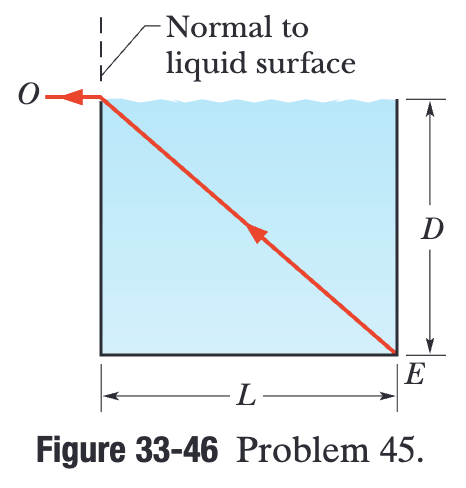
\includegraphics[width=0.33\textwidth]{33-46.png} 
            % \label{fig:wrapfig}
        \end{wrapfigure}
        When the rectangular metal tank in Fig. 33-46 is filled to the top with an unknown liquid, observer O, with eyes level with the top of the tank, can just see corner E. 
        A ray that refracts toward O at the top surface of the liquid is shown. 
        If D = 85.0 cm and L = 1.10 m, what is the index of refraction of the liquid?

        \subsection{Solution}
            Recall Snell's Law.
            \begin{equation}
                n_2 \sin \theta_2 = n_1 \sin \theta_1
            \end{equation}

            The index of refraction of air is $n_1 = 1.00029$, while the angle we use for in the air is going to be $\frac{\pi}{2}$, making $\sin \theta_2 = 1$.
            The distance traveled along the diagonal can be found using the Pythagorean Theorem, which can in turn be used to find the sine of the angle.
            \begin{gather}
                H = \sqrt{D^2 + L^2}\\
                \sin(\theta_1) = \frac{D}{H} = \frac{L}{\sqrt{D^2 + L^2}}
            \end{gather}

            From here, we can find the index of refraction.
            \begin{gather}
                n_2 \sin \theta_2 = n_1 \sin \theta_1\\
                \begin{align}
                    n_2 &=  \frac{n_1 \sin \theta_1}{\sin \theta_2}
                        =   n_1 \frac{\sqrt{D^2 + L^2}}{L}\\
                        &=  1.00029 * \frac{\sqrt{0.85^2 + 1.10^2}}{1.10}
                        =   \boxed{1.264}
                \end{align}
            \end{gather}

    \pagebreak
    \section{Problem 49}
        \begin{wrapfigure}{r}{0.33\textwidth}
            \vspace{-30pt}
            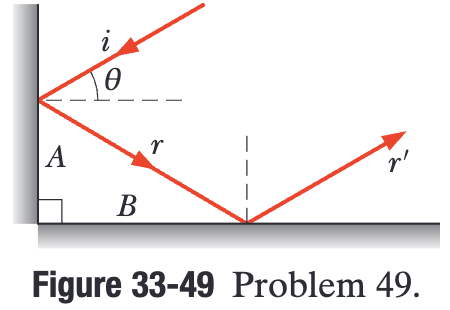
\includegraphics[width=0.33\textwidth]{33-49.png} 
            % \label{fig:wrapfig}
        \end{wrapfigure}
        Figure 33-49 shows light reflecting from two perpendicular reflecting surfaces A and B. 
        Find the angle between the incoming ray $i$ and the outgoing ray $r'$.

        \subsection{Solution}
            Easy. \boxed{180\unit{\degree}}.

    \pagebreak
    \section{Problem 51}
        \begin{wrapfigure}{r}{0.33\textwidth}
            \vspace{-60pt}
            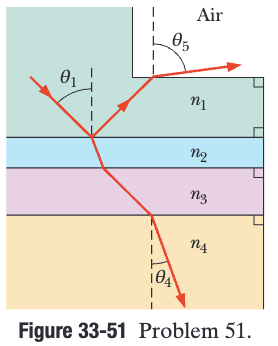
\includegraphics[width=0.33\textwidth]{33-51.png} 
            % \label{fig:wrapfig}
        \end{wrapfigure}
        In Fig. 33-51, light is incident at angle $\theta_1 = 40.1\unit{\degree}$ on a boundary between two transparent materials. 
        Some of the light travels down through the next three layers of transparent materials, while some of it reflects upward and then escapes into the air. 
        If $n_1 = 1.30$, $n_2 = 1.40$, $n_3 = 1.32$, and $n_4 = 1.45$, what is the value of (a) $\theta_5$ in the air and (b) $\theta_4$ in the bottom material?

        \subsection{Solution (a)}
            It will hit the boundary between $n_1$ and the air at the same angle as it hits the boundary between $n_1$ and $n_2$, so we can use the respective version of that angle for $\theta_i$ in Snell's Law.
            \begin{equation}
                n_1
            \end{equation}

    \pagebreak
    \section{Problem 55}
        In Fig. 33-55, a 2.00-m-long vertical pole extends from the bottom of a swimming pool to a point 50.0 cm above the water.
        Sunlight is incident at angle $\theta = 55.0\unit{\degree}$. What is the length of the shadow of the pole on the level bottom of the pool?

        \subsection{Solution}

    \pagebreak
    \section{Problem 59}
        In Fig. 33-57, a ray of light is perpendicular to the face ab of a glass prism (n = 1.52).
        Find the largest value for the angle $\phi$ so that the ray is totally reflected at face ac if the prism is immersed (a) in air and (b) in water.

        \subsection{Solution}

    \pagebreak
    \section{Problem 65}
        Figure 33-61 depicts a simplistic optical fiber: a plastic core ($n_1 = 1.58$) is surrounded by a plastic sheath ($n_2 = 1.53$). 
        A light ray is incident on one end of the fiber at angle $\theta$. 
        The ray is to undergo total internal reflection at point A, where it encounters the core-sheath boundary. 
        (Thus there is no loss of light through that boundary.) 
        What is the maximum value of $\theta$ that allows total internal reflection at A?

        \subsection{Solution}

    \pagebreak
    \section{Problem 69}
        Light that is traveling in water (with an index of refraction of 1.33) is incident on a plate of glass (with index of refraction 1.53). 
        At what angle of incidence does the reflected light end up fully polarized?

        \subsection{Solution}

    \pagebreak
    \section{Problem 71}

        \subsection{Solution}

    \pagebreak
    \section{Problem 75}

        \subsection{Solution}

    \pagebreak
    \section{Problem 83}

        \subsection{Solution}

    \pagebreak
    \section{Problem 87}

        \subsection{Solution}

    \pagebreak
    \section{Problem 89}

        \subsection{Solution}

    \pagebreak
    \section{Problem 91}

        \subsection{Solution}

    \pagebreak
    \section{Problem 105}

        \subsection{Solution}

    \pagebreak
    \tableofcontents
\end{document}